
% ----------------------------------------------------------
\chapter{Metodologia de calibração utilizando as leituras de todos os sensores}\label{cap:calib-methodology}
% ----------------------------------------------------------

No Capítulo \ref{cap:field-monit-results} foram apresentados os resultados de aplicar modelos de regressão nas leituras dos sensores de gases para inferir a concentração real de cada poluente. Neles foram consideradas como variáveis de entrada de cada modelo a temperatura e as leituras do(s) sensor(es) especificados para cada composto gasoso. Assim, foram utilizados um sensor CO-B4 e a temperatura para medir \acrshort{co}; dois sensores OX-B431 e a temperatura para medir \acrshort{o3}; e um sensor NO2-B43F para medir \acrshort{no2}. No presente capítulo, serão aplicada uma metodologia de calibração similar ã do capítulo \ref{cap:field-monit-results}, mas dessa vez serão consideradas as leituras de todos os sensores para inferir a concentração de cada gás. Serão aplicadas buscas em grid para avaliar as combinações de variáveis de entrada e de parâmetros que produzam os melhores resultados de R2 e erro. Como a complexidade dos modelos aumenta com o incremento das variáveis independentes, também serão considerados as métricas de \acrshort{aic} e \acrshort{bic} na avaliação dos modelos de regressão.

% ----------------------------------------------------------
\section{Correção das leituras do sensor CO-B4 com as medições de referência}
% ----------------------------------------------------------

A partir dos dados de referência e das leituras de concentração e temperatura adquiridas pelo monitor em questão, foi realizada uma busca em \textit{grid} para encontrar as melhores combinações de parâmetros e variáveis de entrada aos modelos de regressão. As variáveis que foram testadas como entrada foram as leituras de concentração do sensor CO-B4 e a temperatura no interior da câmara de medição. Na Tabela \ref{tab:data-co-br-calib-results} resumem-se os melhores modelos encontrados pela busca em \textit{grid} para corrigir as leituras do sensor CO-B4. Os mesmos resultados são ilustrados graficamente na Figura \ref{fig:data-co-b4-models-performance} que apresenta o desempenho dos modelos e as variáveis de entrada considerando os valores de r2, RMSE e MAE.

\begin{table}[h!]
    \caption{Resultados da calibração do sensor CO-B4}
    \centering
    \begin{tabularx}{0.95\textwidth}[h!]{
         >{\raggedright\hsize=.2\hsize\arraybackslash}X
         >{\raggedright\hsize=.7\hsize\arraybackslash}X 
         >{\raggedright\hsize=.4\hsize\arraybackslash}X
         >{\raggedright\hsize=.4\hsize\arraybackslash}X 
         >{\raggedright\hsize=.3\hsize\arraybackslash}X 
         >{\raggedright\hsize=.3\hsize\arraybackslash}X }
        \hline
        Var. & Modelo & R2 & RMSE & MAE & $\rho$\\ [0.5ex]
        \hline
        CO & \textbf{MLP}: & -0.45 ± 0.25 & -0.06 ± 0.01 & -0.05 & 0.47 \\ [0.5ex]
           & \textbf{MLR} & -0.63 ± 0.48 & -0.07 ± 0.01 & -0.05 & 0.33 \\ [0.5ex]
           & \textbf{KNN:} & -0.48 ± 0.29 & -0.06 ± 0.01 & -0.05 & 0.46 \\ [0.5ex]
           & \textbf{RF:} & -0.61 ± 0.35 & -0.07 ± 0.01 & -0.05 & 0.39 \\ [0.5ex]
        \hline
        CO, T & \textbf{MLP:} & -0.65 ± 0.40 & -0.07 ± 0.01 & -0.05 ± 0.01 & 0.50 \\ [0.5ex]
              & \textbf{MLR:} & -0.68 ± 0.47 & -0.07 ± 0.01 & -0.05 & 0.31 \\ [0.5ex]
              & \textbf{KNN:} & -0.63 ± 0.38 & -0.07 ± 0.01 & -0.05 & 0.53 \\ [0.5ex]
              & \textbf{RF:} & -0.63 ± 0.43 & -0.07 ± 0.01 & -0.05 & 0.47 \\ [0.5ex]
        \hline
    \end{tabularx}
    \label{tab:data-co-br-calib-results}
\end{table}

\begin{figure}[h]
    \centering
    \caption{Resultados dos modelos de regressão aplicados as leituras do sensor CO-B4}
    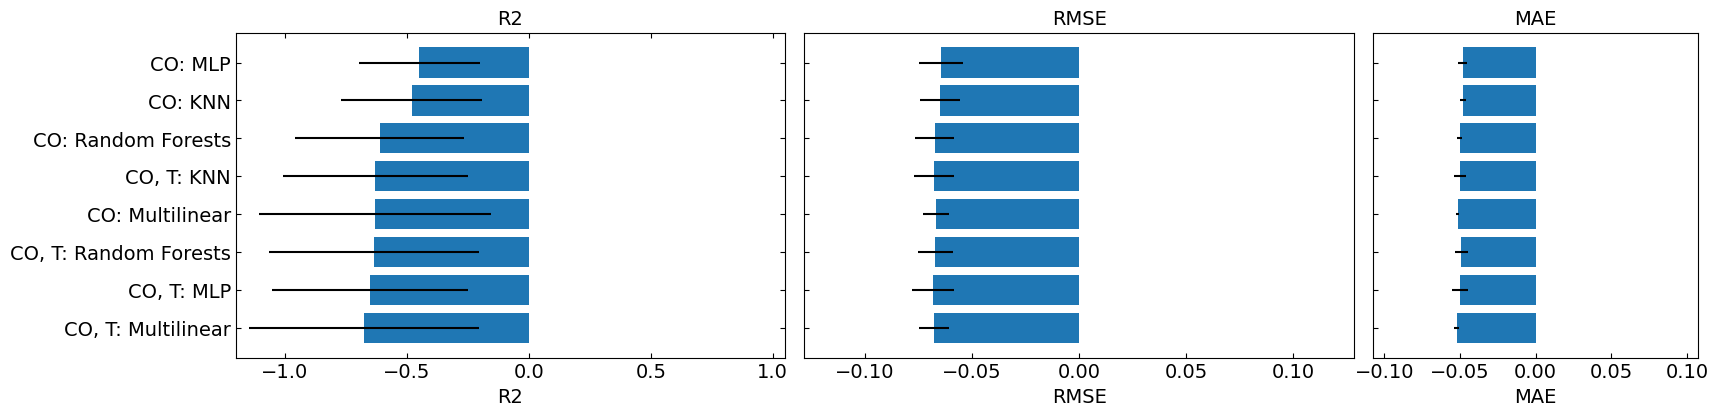
\includegraphics[width=\textwidth]{chapters/4-CALIBRAÇÃO MÚLTIPLOS SENSORES/Figuras/co-b4-models-performance.png}
    \label{fig:data-co-b4-models-performance}
\end{figure}

Como se observa, todas as variantes de modelos e variáveis de entrada apresentaram valores de R2 negativos, indicando que nenhum dos modelos foi capaz de explicar a variância na variável dependente, i.e. a concentração real. Contudo, os modelos não lineares produziram maiores coeficientes de correlação do que as regressões lineares, e de igual modo, os modelos não lineares que incluíram a temperatura, apresentaram melhorias na correlação em comparação com os que não consideraram a temperatura como variável de entrada. Os maiores coeficientes de Spearman foram de 0.53 com uma regressão KNN considerando a temperatura, e de 0.50 utilizando uma rede neural MLP também considerando a temperatura. As Figuras \ref{fig:data-co-T-reference-corr-KNN} e \ref{fig:data-co-T-reference-corr-MLP} apresentam os resultados ao aplicar os modelos de k Vizinhos mais Próximos e Perceptron Multicamadas.

\begin{figure}[h]
    \centering
    \caption{Gráfico de dispersão das leituras do sensor CO-B4 e a estação de referência após aplicar modelos de regressão considerando a temperatura}
    \begin{subfigure}{0.495\textwidth}
        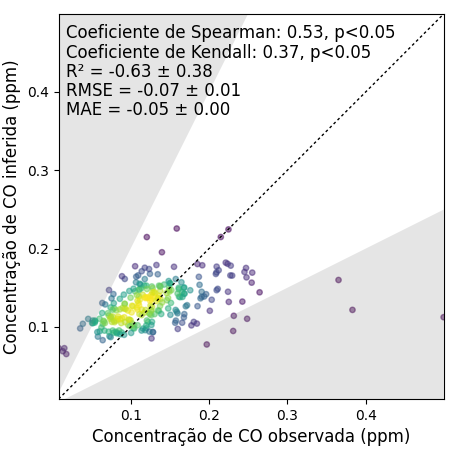
\includegraphics[width=\textwidth]{chapters/4-CALIBRAÇÃO MÚLTIPLOS SENSORES/Figuras/co-b4-T-KNN-Regression.png}
        \caption{Utilizando regressão pelos k Vizinhos mais Próximos}
        \label{fig:data-co-T-reference-corr-KNN}
    \end{subfigure}
    \hfill
    \begin{subfigure}{0.495\textwidth}
        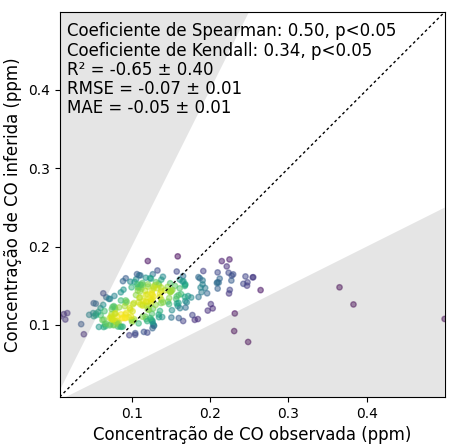
\includegraphics[width=\textwidth]{chapters/4-CALIBRAÇÃO MÚLTIPLOS SENSORES/Figuras/co-b4-T-MLP-Regression.png}
        \caption{Utilizando uma rede neural Perceptron Multicamadas}
        \label{fig:data-co-T-reference-corr-MLP}
    \end{subfigure}
\end{figure}

\begin{figure}[h!]
    \centering
    \caption{Desempenho dos modelos de regressão aplicados para inferir as leituras de concentração de \acrshort{co} medidas pela estação de referência}
    \begin{subfigure}{\textwidth}
        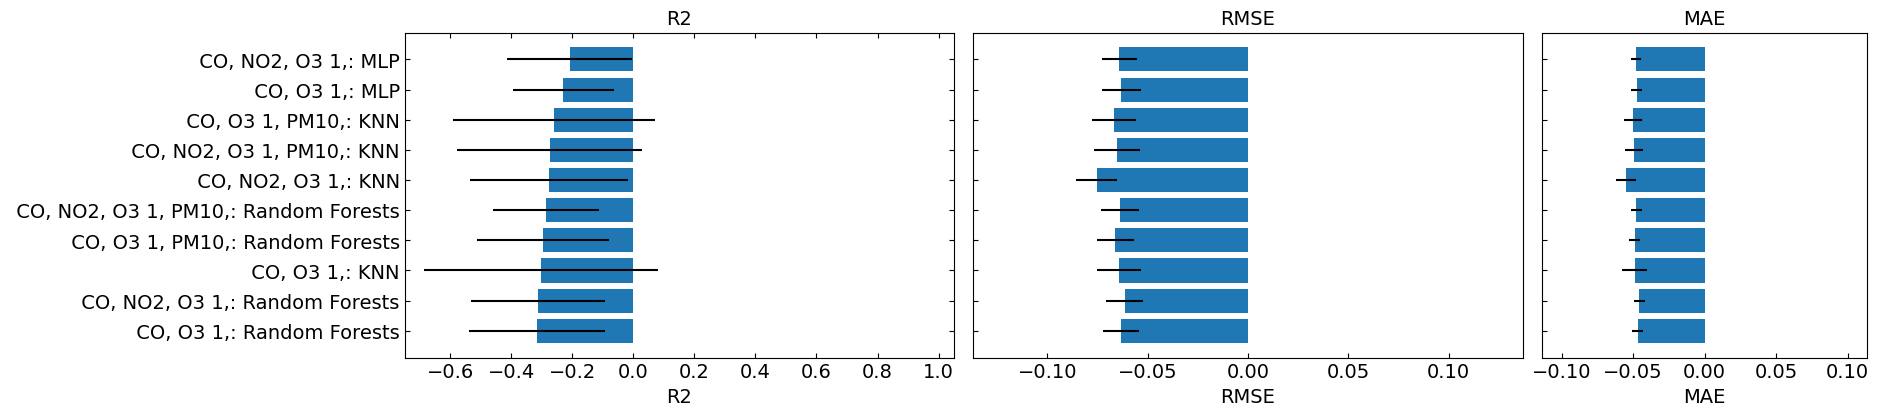
\includegraphics[width=\textwidth]{chapters/4-CALIBRAÇÃO MÚLTIPLOS SENSORES/Figuras/co-all-models-performance.png}
        \caption{Valores de R2, RMSE e MAE obtidos pelos 10 modelos com maiores valores de R2}
        \label{fig:data-co-all-models-performance}
    \end{subfigure}
    \begin{subfigure}{\textwidth}
        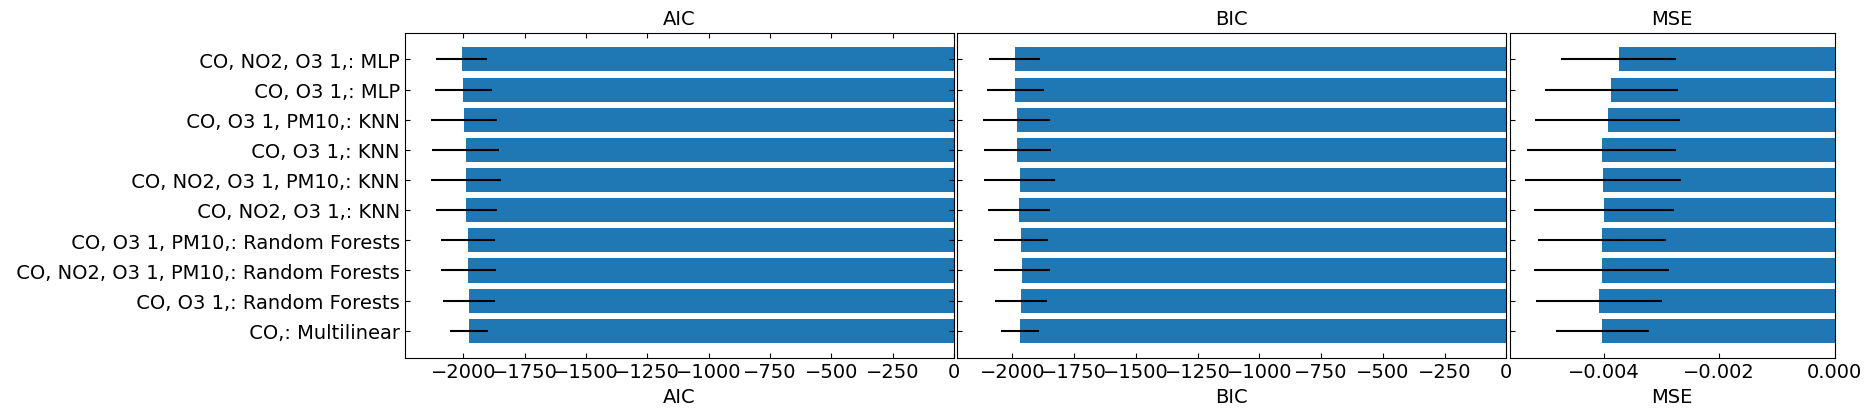
\includegraphics[width=\textwidth]{chapters/4-CALIBRAÇÃO MÚLTIPLOS SENSORES/Figuras/co-all-models-complexity.png}
        \caption{Modelos com menores valores de \acrshort{aic} e \acrshort{bic}}
        \label{fig:data-co-all-models-complexity}
    \end{subfigure}
    \label{fig:data-co-all-models-performance-comlexity}
\end{figure}

% ----------------------------------------------------------
\section{Cálculo da concentração de Monóxido de Carbono a partir das leituras do arranjo de sensores de gases}
% ----------------------------------------------------------

A Figura \ref{fig:data-co-all-models-performance} apresenta os valores de R2 dos 10 melhores modelos de calibração calculados para as leituras de \acrshort{co}. Observa-se que apesar do valor médio de R2 obtido nas validações cruzadas continuar sendo negativo, obtiveram-se máximos de até aproximadamente 0.1 para alguns conjuntos de dados de teste nas validações cruzadas. Em geral os modelos que produziram os melhores resultados foram baseados em regressões pelos k vizinhos mais próximos e redes neurais Perceptron Multicamadas. Com relação as variáveis de entrada dos modelos, todos os que produziram melhores resultados consideraram as leituras do sensor 1 de \acrshort{o3}. Nenhum deles considerou a temperatura.

\begin{figure}[h!]
    \centering
    \caption{Gráfico de dispersão das leituras do múltiplos sensores e a estação de referência para medição de \acrshort{co}}
    \begin{subfigure}{0.495\textwidth}
        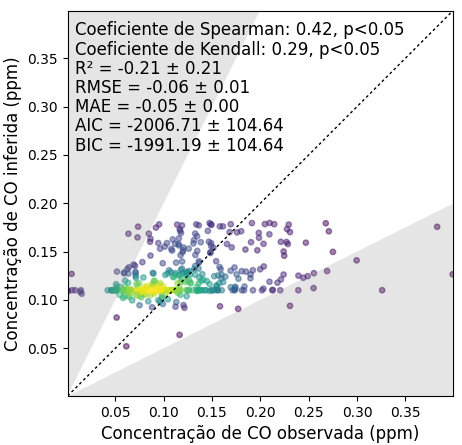
\includegraphics[width=\textwidth]{chapters/4-CALIBRAÇÃO MÚLTIPLOS SENSORES/Figuras/CO-co-no2-o31-mlp-Regression.png}
        \caption{Utilizando modelo de regressão com uma rede neural Perceptron Multicamadas; variáveis independentes: leituras de sensores CO-B4, NO2-B43F e OX-B431 (1)}
        \label{fig:data-co-no2-o31-reference-corr-MLP}
    \end{subfigure}
    \hfill
    \begin{subfigure}{0.495\textwidth}
        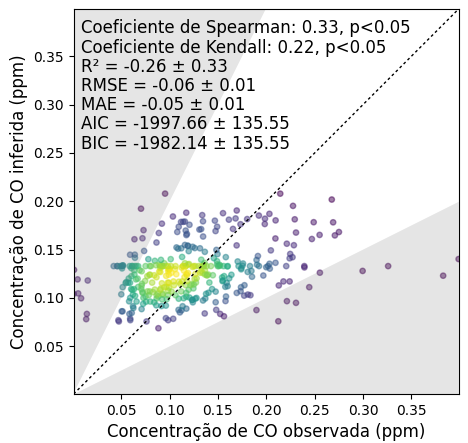
\includegraphics[width=\textwidth]{chapters/4-CALIBRAÇÃO MÚLTIPLOS SENSORES/Figuras/CO-co-o31-pm10-knn-Regression.png}
        \caption{Utilizando modelo de regressão pelos k vizinhos mais próximos; variáveis independentes: leituras de sensores CO-B4, OX-B431 (1) e de \acrshort{mp10} medido pelo OPC-N3}
        \label{fig:data-co-o31-mp10-reference-corr-KNN}
    \end{subfigure}
\end{figure}

Ao comparar os modelos em termos de sua complexidade, observa-se uma sobreposição entre os que desempenharam melhor em termos de representação dos dados originais (maiores valores de R2) e os que desempenharam melhor em termos de complexidade (menores valores de AIC e BIC). A Figura \ref{fig:data-co-all-models-complexity} compara os valores de \acrshort{aic}, \acrshort{bic} e \acrshort{mse} dos 10 modelos que obtiveram menores valores de AIC. Por último as Figuras \ref{fig:data-co-no2-o31-reference-corr-MLP} e \ref{fig:data-co-o31-mp10-reference-corr-KNN} mostram gráficos de dispersão entre os valores de saída dos modelos de calibração e os dados de referência de \acrshort{co}. Os gráficos mostram os resultados dos modelos com melhores valores de R2.

% ----------------------------------------------------------
\section{Calibração das leituras de Ozônio}
% ----------------------------------------------------------

\begin{figure}[h!]
    \centering
    \caption{Desempenho dos modelos de regressão aplicados para inferir as leituras de concentração de \acrshort{o3} medidas pela estação de referência}
    \begin{subfigure}{0.9\textwidth}
        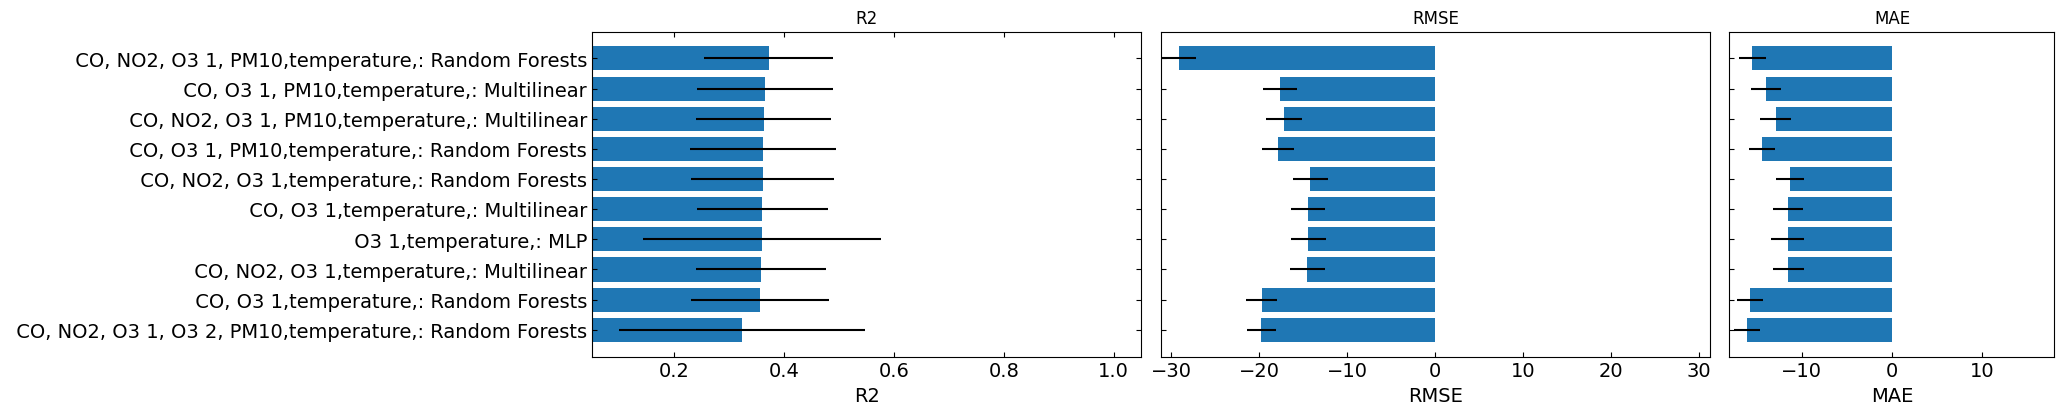
\includegraphics[width=\textwidth]{chapters/4-CALIBRAÇÃO MÚLTIPLOS SENSORES/Figuras/o3-all-models-performance.png}
        \caption{Valores de R2, RMSE e MAE obtidos pelos 10 modelos com maiores valores de R2}
        \label{fig:data-o3-all-models-performance}
    \end{subfigure}
    \begin{subfigure}{0.9\textwidth}
        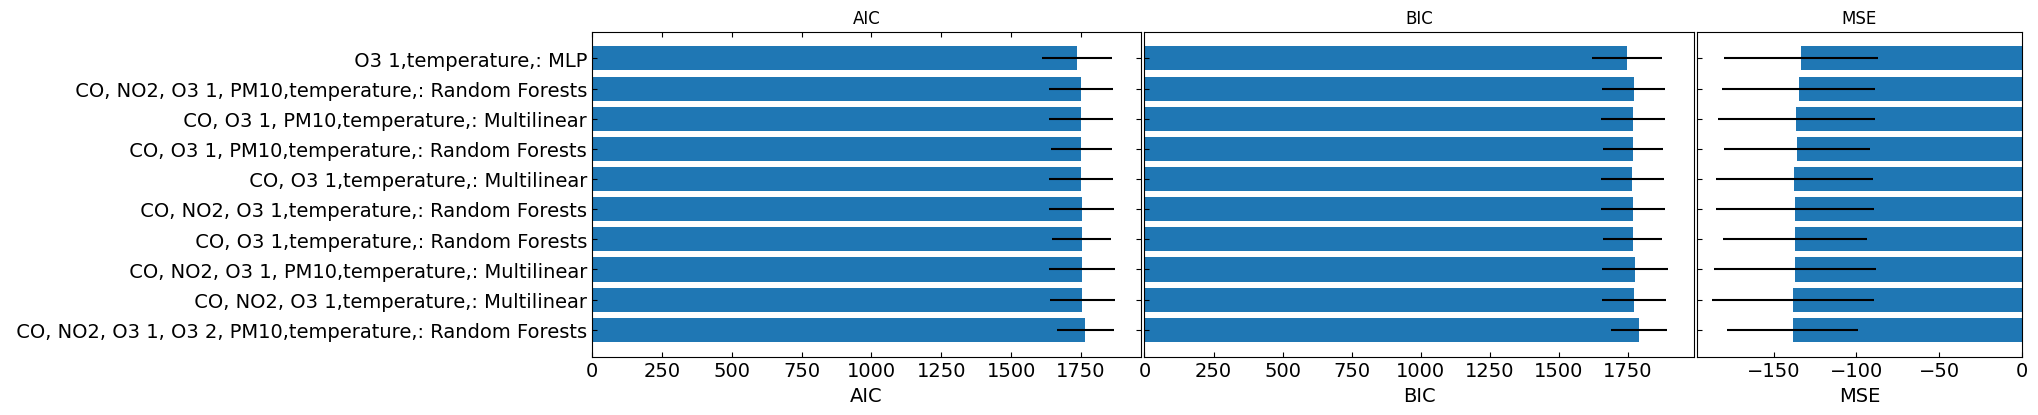
\includegraphics[width=\textwidth]{chapters/4-CALIBRAÇÃO MÚLTIPLOS SENSORES/Figuras/o3-all-models-complexity.png}
        \caption{Modelos com menores valores de \acrshort{aic} e \acrshort{bic}}
        \label{fig:data-o3-all-models-comlexity}
    \end{subfigure}
    \label{fig:data-o3-all-models-performance-comlexity}
\end{figure}

A Figura \ref{fig:data-o3-all-models-performance} apresenta os valores de R2 dos 10 melhores modelos de calibração calculados para as leituras de \acrshort{co}. Observa-se que os valores de R2 desses 10 modelos oscilaram entre 0.2 e 0.6, todos incluíram o \acrshort{co} e a temperatura. Apenas dois modelos não foram regressões lineares, ocupando as posições 5 e 6 com regressões por Florestas Aleatórias. As Florestas, embora não tenham produzido os maiores valores de R2 médio, apresentaram menores valores de erro e valores de R2 máximo mais altos em comparação com os quatro modelos lineares que os antecederam. Já em termos de complexidade, observa-se que apenas o modelo de regressão por Florestas Aleatórias que considerou como variáveis de entrada as leituras de \acrshort{co}, dos dois sensores de \acrshort{o3}, de \acrshort{mp10} e temperatura, conseguiu estar entre os 10 com menores valores de \acrshort{aic}. Os modelos lineares por sua parte produziram os menores coeficientes de complexidade.

\begin{figure}[h]
    \centering
    \caption{Gráfico de dispersão das leituras do múltiplos sensores e a estação de referência para medição de \acrshort{o3}}
    \begin{subfigure}{0.49\textwidth}
        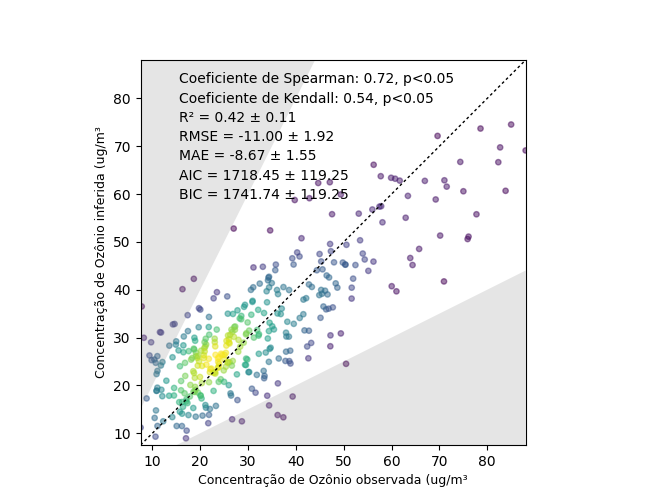
\includegraphics[width=\textwidth]{chapters/4-CALIBRAÇÃO MÚLTIPLOS SENSORES/Figuras/O3-co-no2-o31-pm10-T-Multilinear-Regression.png}
        \caption{Utilizando modelo de regressão linear multivariado com variáveis independentes: leituras de sensores CO-B4, NO2-B43F, OX-B431 (1), sensor de \acrshort{mp10} OPC-N3 e temperatura}
        \label{fig:data-co-no2-o31-pm10-T-reference-O3-corr-MLR}
    \end{subfigure}
    \hfill
    \begin{subfigure}{0.49\textwidth}
        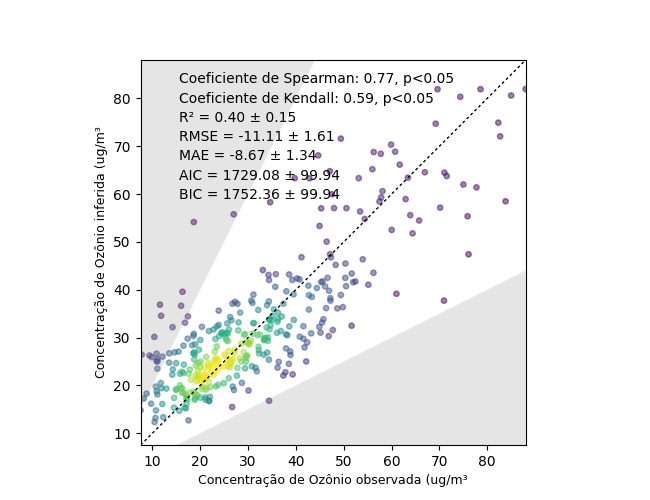
\includegraphics[width=\textwidth]{chapters/4-CALIBRAÇÃO MÚLTIPLOS SENSORES/Figuras/O3-co-o31-o32-pm10-T-RF-Regression.png}
        \caption{Utilizando modelo de regressão de Florestas Aleatórias com variáveis independentes: leituras de sensores CO-B4, OX-B431 (1 e 2), sensor de \acrshort{mp10} OPC-N3 e temperatura}
        \label{fig:data-co-o31-o32-pm10-T-reference-O3-corr-RF}
    \end{subfigure}
\end{figure}

As Figuras \ref{fig:data-co-no2-o31-pm10-T-reference-O3-corr-MLR} e \ref{fig:data-co-o31-o32-pm10-T-reference-O3-corr-RF} mostram os resultados de aplicar modelos de calibração baseados numa regressão linear multivariada e em Florestas Aleatórias respectivamente. O primeiro considera como variáveis independentes as leituras dos sensores CO-B4, NO2-B43F, OX-B431 (1), sensor de \acrshort{mp10} OPC-N3 e temperatura. Já o segundo considera como variáveis de entrada as leituras dos sensores CO-B4, OX-B431 (1 e 2), sensor de \acrshort{mp10} OPC-N3 e temperatura.

\begin{table}[h!]
    \caption{Resultados da calibração das leituras de \acrshort{no2} do sensor NO2-B43F}
    \centering
    \begin{tabularx}{0.95\textwidth}[h!]{
        >{\raggedright\hsize=.4\hsize\arraybackslash}X
        >{\raggedright\hsize=.6\hsize\arraybackslash}X 
        >{\raggedright\hsize=.6\hsize\arraybackslash}X
        >{\raggedright\hsize=.7\hsize\arraybackslash}X 
        >{\raggedright\hsize=.6\hsize\arraybackslash}X 
        >{\raggedright\hsize=.3\hsize\arraybackslash}X }
        \hline
        Var. & Modelo & R2 & RMSE & MAE & $\rho$\\ [0.5ex]
        \hline
        \acrshort{no2} & \textbf{MLP}: & -3.95 ± 5.68 & -12.87 ± 3.90 & -9.94 ± 2.52 & -- \\ [0.5ex]
           & \textbf{MLR} & -3.80 ± 6.39 & -12.61 ± 3.74 & -9.62 ± 2.17 & -- \\ [0.5ex]
           & \textbf{KNN:} & -3.73 ± 5.49 & -12.84 ± 3.67 & -9.92 ± 2.10 & -- \\ [0.5ex]
           & \textbf{RF:} & -4.39 ± 6.07 & -13.70 ± 3.50 & -10.33 ± 2.08 & -- \\ [0.5ex]
        \hline
        \acrshort{no2}, T & \textbf{MLP:} & -2.84 ± 4.36 & -11.76 ± 3.40 & -9.00 ± 1.81 & 0.59 \\ [0.5ex]
              & \textbf{MLR:} & -3.62 ± 5.88 & -12.57 ± 3.40 & -9.70 ± 1.87 & -- \\ [0.5ex]
              & \textbf{KNN:} & -2.62 ± 4.52 & -12.02 ± 3.33 & -8.88 ± 1.54 & 0.61 \\ [0.5ex]
              & \textbf{RF:} & -2.66 ± 4.51 & -11.93 ± 3.39 & -9.18 ± 2.03 & 0.63 \\ [0.5ex]
        \hline
    \end{tabularx}
    \label{tab:data-no2-calib-results}
\end{table}

% ----------------------------------------------------------
\section{Correção das leituras do sensor NO2-B43F com as medições de referência}
% ----------------------------------------------------------

A partir dos dados de referência e das leituras de concentração e temperatura adquiridas pelo monitor em questão, foi realizada uma busca em grid para encontrar as melhores combinações de parâmetros e variáveis de entrada a modelos de regressão. As variáveis que foram testadas como entrada foram as leituras de concentração de \acrshort{no2} do sensor NO2-B43F e a temperatura no interior da câmara de medição. Como modelos de regressão foram testados: o Perceptron Multicamadas (MLP), a Regressão Linear Multivariada (MLR), os K Vizinhos mais Próximos (KNN) e as Florestas Aleatórias (RF). Na Tabela \ref{tab:data-no2-calib-results} resumem-se os melhores modelos encontrados pela busca em \textit{grid} para calibrar as leituras do sensor de baixo custo. Os mesmos resultados são ilustrados graficamente na Figura \ref{fig:data-no2-models-performance} que apresenta o desempenho dos modelos e as variáveis de entrada considerando os valores de R2, RMSE e MAE.

\begin{figure}[h!]
    \centering
    \caption{Resultados dos modelos de calibração aplicados as leituras de \acrshort{no2} do sensor NO2-B43F}
    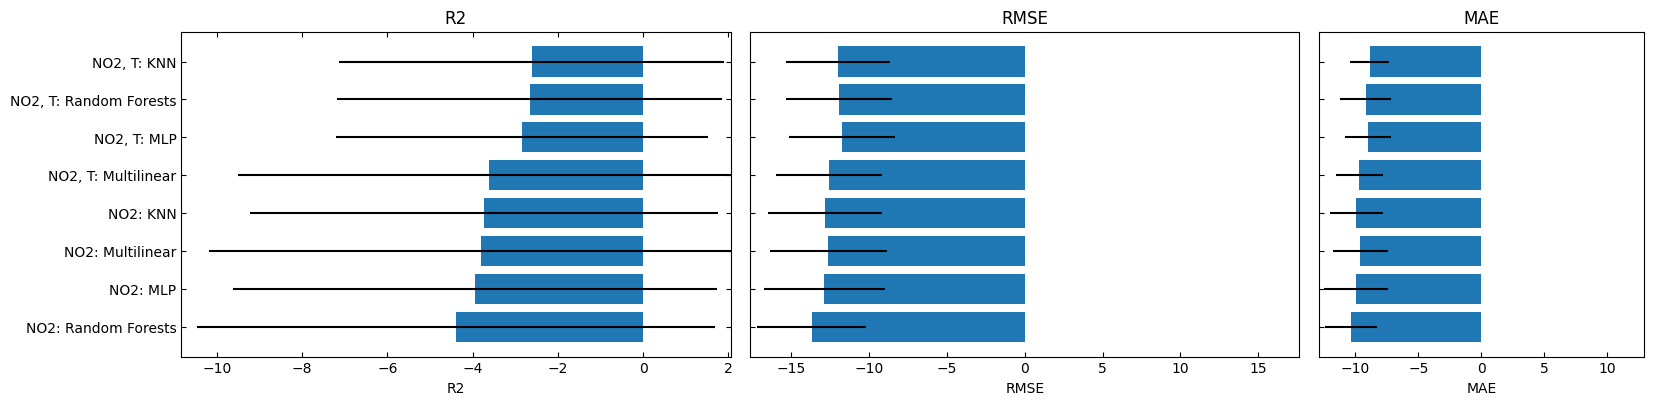
\includegraphics[width=0.95\textwidth]{chapters/4-CALIBRAÇÃO MÚLTIPLOS SENSORES/Figuras/no2-B43F-models-performance.png}
    \label{fig:data-no2-models-performance}
\end{figure}

\begin{figure}[h!]
    \centering
    \caption{Gráfico de dispersão das leituras do sensor de \acrshort{no2} NO2-B43F e a estação de referência após aplicar modelos de regressão considerando a temperatura}
    \begin{subfigure}{0.49\textwidth}
        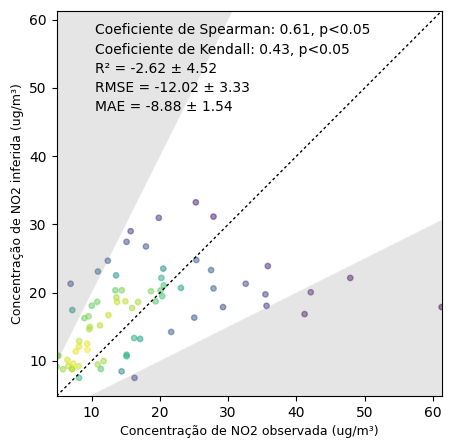
\includegraphics[width=\textwidth]{chapters/4-CALIBRAÇÃO MÚLTIPLOS SENSORES/Figuras/no2-T-KNN-Regression.png}
        \caption{Utilizando uma regressão pelos k vizinhos mais próximos considerando a temperatura obteve-se um $\rho$ de 0.61}
        \label{fig:data-no2-T-reference-corr-KNN}
    \end{subfigure}
    \hfill
    \begin{subfigure}{0.49\textwidth}
        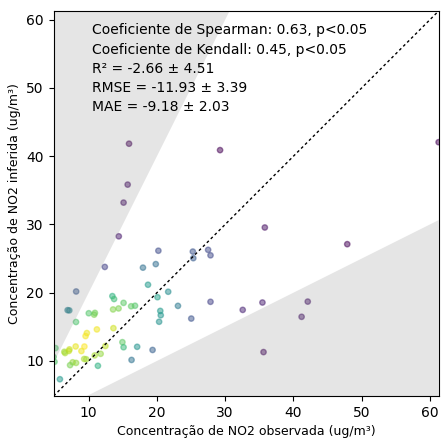
\includegraphics[width=\textwidth]{chapters/4-CALIBRAÇÃO MÚLTIPLOS SENSORES/Figuras/no2-T-RF-Regression.png}
        \caption{Utilizando uma regressão por Florestas Aleatórias considerando a temperatura obteve-se um valor de $\rho$ de 0.63}
        \label{fig:data-no2-T-reference-corr-RF}
    \end{subfigure}
\end{figure}

Como se observa todas as variantes de modelos e variáveis de entrada apresentaram valores de R2 negativos, indicando que nenhum dos modelos foi capaz de explicar a variância na variável dependente, i.e. a concentração real. Observa-se também que nenhum dos modelos uni-variados conseguiu que os dados observados e os inferidos apresentassem alguma correlação. Por outro lado, os modelos multivariados, a exceção da regressão linear, que incluíram a temperatura como variável de entrada, produziram coeficientes de correlação entre a concentração real e a medida pelo sensor, entre 0.59 - 0.63. As Figuras \ref{fig:data-no2-T-reference-corr-KNN} e \ref{fig:data-no2-T-reference-corr-RF} apresentam os resultados ao aplicar os modelos de k Vizinhos mais Próximos e Florestas Aleatórias.

\begin{figure}[h!]
    \centering
    \caption{Desempenho dos modelos de regressão aplicados para inferir as leituras de concentração de \acrshort{no2} medidas pela estação de referência}
    \begin{subfigure}{0.9\textwidth}
        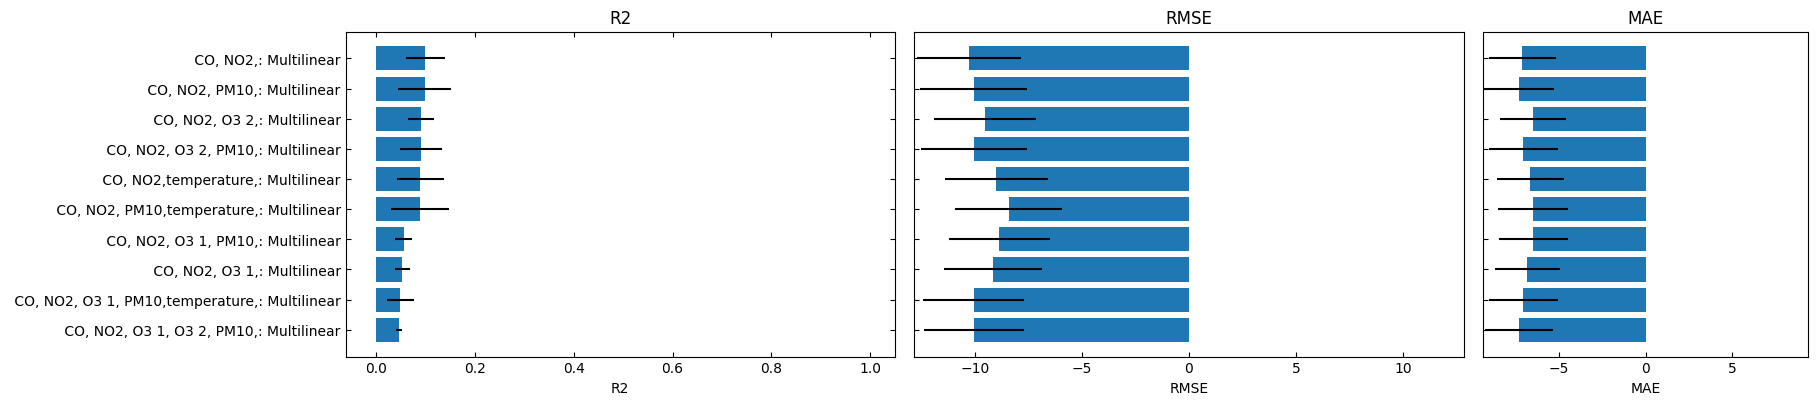
\includegraphics[width=\textwidth]{chapters/4-CALIBRAÇÃO MÚLTIPLOS SENSORES/Figuras/no2-all-models-performance.png}
        \caption{Valores de R2, RMSE e MAE obtidos pelos 10 modelos com maiores valores de R2}
        \label{fig:data-no2-all-models-performance}
    \end{subfigure}
    \begin{subfigure}{0.9\textwidth}
        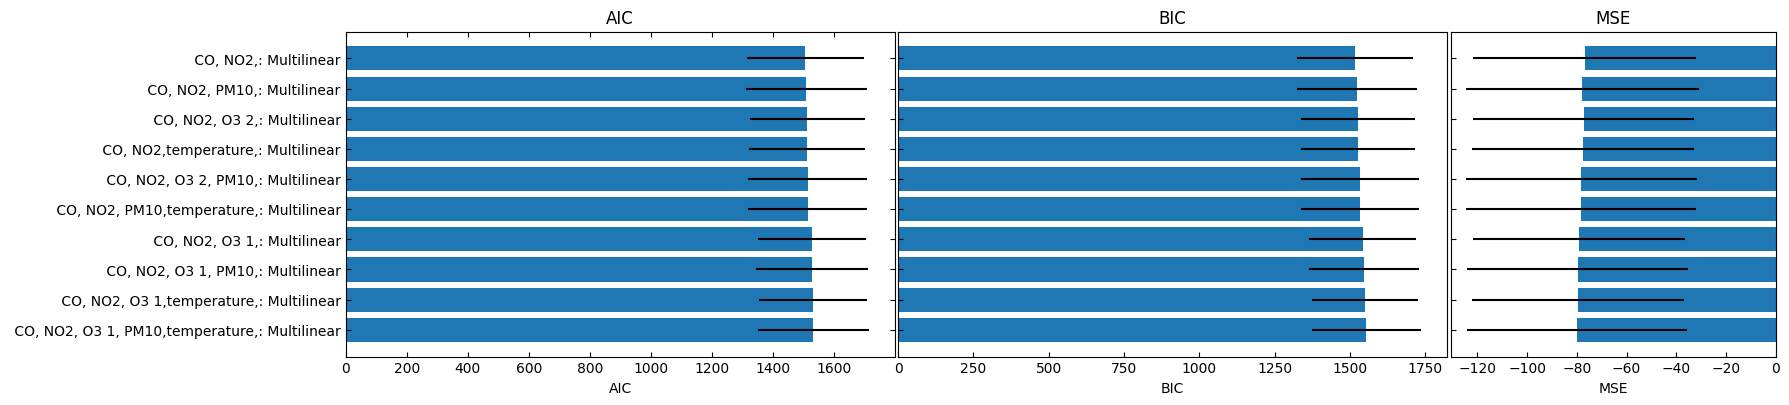
\includegraphics[width=\textwidth]{chapters/4-CALIBRAÇÃO MÚLTIPLOS SENSORES/Figuras/no2-all-models-complexity.png}
        \caption{Modelos com menores valores de \acrshort{aic} e \acrshort{bic}}
        \label{fig:data-no2-all-models-comlexity}
    \end{subfigure}
    \label{fig:data-no2-all-models-performance-comlexity}
\end{figure}

\begin{figure}[h]
    \centering
    \caption{Gráfico de dispersão das leituras de múltiplos sensores e a estação de referência para medição de \acrshort{no2}}
    \begin{subfigure}{0.49\textwidth}
        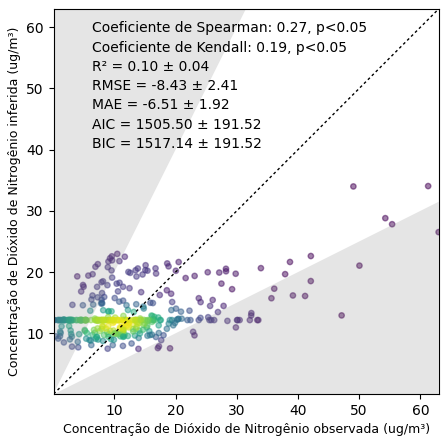
\includegraphics[width=\textwidth]{chapters/4-CALIBRAÇÃO MÚLTIPLOS SENSORES/Figuras/NO2-co-no2-Multilinear-Regression.png}
        \caption{Utilizando modelo de regressão linear multivariado com variáveis independentes: leituras de sensores CO-B4, e NO2-B43F}
        \label{fig:data-co-no2-reference-NO2-corr-MLR}
    \end{subfigure}
    \hfill
    \begin{subfigure}{0.49\textwidth}
        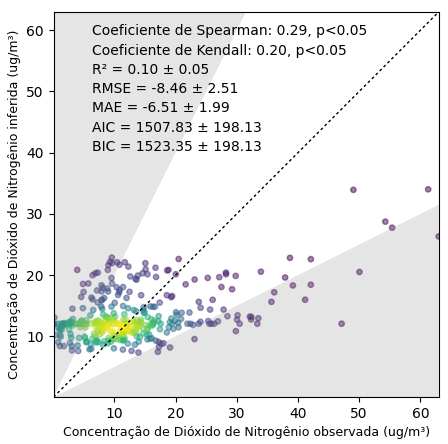
\includegraphics[width=\textwidth]{chapters/4-CALIBRAÇÃO MÚLTIPLOS SENSORES/Figuras/NO2-co-no2-pm10-Multilinear-Regression.png}
        \caption{Utilizando modelo de regressão linear multivariado com variáveis independentes: leituras de sensores CO-B4, NO2-B43F e sensor de \acrshort{mp10} OPC-N3}
        \label{fig:data-co-no2-pm10-reference-NO2-corr-RF}
    \end{subfigure}
\end{figure}

% ----------------------------------------------------------
\section{Cálculo da concentração de Dióxido de Nitrogênio a partir das leituras do arranjo de sensores de gases}
% ----------------------------------------------------------

A Figura \ref{fig:data-no2-all-models-performance} apresenta os valores de R2 dos 10 melhores modelos de calibração calculados para as leituras de \acrshort{no2}. Observa-se que os valores de R2 desses 10 modelos apresentaram valores de R2 em média positivos, com valores máximos de até aproximadamente 0.2, todos obtidos a partir de regressões lineares. Com relação as variáveis de entrada observa-se que todos os 10 modelos consideraram o \acrshort{co} com variações nos restantes das variáveis para cada modelo. Com relação à complexidade dos modelos (Figura \ref{fig:data-no2-all-models-performance-comlexity}) observa-se que o ranqueamento por \acrshort{aic} coincidiu bastante com o ranqueamento por R2. As Figuras \ref{fig:data-co-no2-reference-NO2-corr-MLR} e \ref{fig:data-co-no2-pm10-reference-NO2-corr-RF} mostram os resultados obtidos com os dois modelos com maior R2 médio, i.e.: regressões lineares com variáveis de entrada leituras de sensores CO-B4 e NO2B43F, e leituras de sensores CO-B4, NO2B43F e sensor de \acrshort{mp10} OPC-N3, respectivamente. As figuras mostram gráficos de dispersão entre os dados calibrados por esses modelos e as leituras de referência.

\begin{table}[h!]
    \caption{Resultados da calibração das leituras de \acrshort{mp10} do sensor OPC-N3}
    \centering
    \begin{tabularx}{0.95\textwidth}[h!]{
        >{\raggedright\hsize=.4\hsize\arraybackslash}X
        >{\raggedright\hsize=.6\hsize\arraybackslash}X 
        >{\raggedright\hsize=.6\hsize\arraybackslash}X
        >{\raggedright\hsize=.7\hsize\arraybackslash}X 
        >{\raggedright\hsize=.6\hsize\arraybackslash}X 
        >{\raggedright\hsize=.3\hsize\arraybackslash}X }
        \hline
        Var. & Modelo & R2 & RMSE & MAE & $\rho$\\ [0.5ex]
        \hline
        \acrshort{mp10} & \textbf{MLP}: & -0.05 ± 0.036 & -9.77 ± 0.75 & -7.41 ± 0.49 & 0.18 \\ [0.5ex]
           & \textbf{MLR} & -0.01 ± 0.03 & -9.57 ± 0.98 & -7.26 ± 0.62 & 0.17 \\ [0.5ex]
           & \textbf{KNN:} & -0.14 ± 0.07 & -10.18 ± 0.62 & -7.71 ± 0.45 & 0.13 \\ [0.5ex]
           & \textbf{RF:} & -0.19 ± 0.11 & -10.33 ± 0.52 & -7.80 ± 0.40 & 0.22\\ [0.5ex]
        \hline
        \acrshort{mp10}, T & \textbf{MLP:} & -0.29 ± 0.27 & -10.68 ± 0.96 & -8.33 ± 0.78 & 0.47 \\ [0.5ex]
              & \textbf{MLR:} & 0.10 ± 0.08 & -9.04 ± 1.12 & -6.73 ± 0.69 & 0.37 \\ [0.5ex]
              & \textbf{KNN:} & -0.02 ± 0.09 & -9.57 ± 0.46 & -7.29 ± 0.27 & 0.45 \\ [0.5ex]
              & \textbf{RF:} & -0.17 ± 0.27 & -10.12 ± 0.32 & -7.89 ± 0.28 & 0.46 \\ [0.5ex]
        \hline
    \end{tabularx}
    \label{tab:data-pm10-calib-results}
\end{table}

% ----------------------------------------------------------
\section{Correção das leituras de MP10 do sensor OPC-N3 com as medições de referência}
% ----------------------------------------------------------

A partir dos dados de referência e das leituras de concentração e temperatura adquiridas pelo monitor em questão, foi realizada uma busca em grid para encontrar as melhores combinações de parâmetros e variáveis de entrada a modelos de regressão. As variáveis que foram testadas como entrada foram as leituras de concentração de \acrshort{mp10} do sensor OPC-N3 e a temperatura no interior da câmara de medição. Como modelos de regressão foram testados: o Perceptron Multicamadas (MLP), a Regressão Linear Multivariada (MLR), os K Vizinhos mais Próximos (KNN) e as Florestas Aleatórias (RF). Na Tabela \ref{tab:data-pm10-calib-results} resumem-se os melhores modelos encontrados pela busca em \textit{grid} para calibrar as leituras do sensor OPC-N3. Os mesmos resultados são ilustrados graficamente na Figura \ref{fig:data-pm10-models-performance} que apresenta o desempenho dos modelos e as variáveis de entrada considerando os valores de r2, RMSE e MAE.

\begin{figure}[h!]
    \centering
    \caption{Resultados dos modelos de calibração aplicados as leituras de \acrshort{mp10} do sensor OPC-N3}
    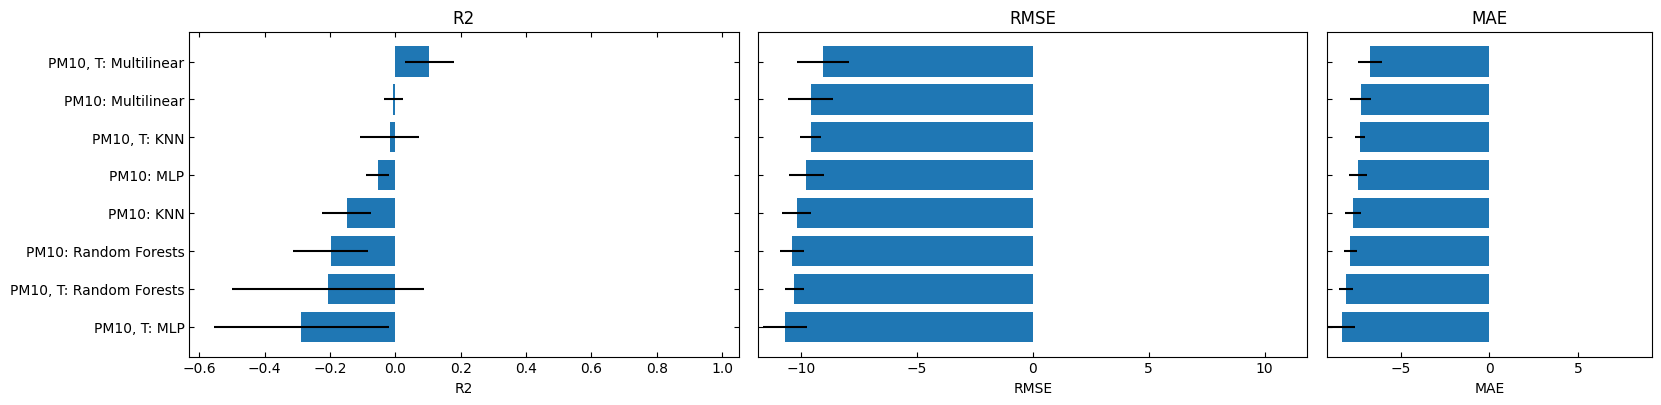
\includegraphics[width=0.95\textwidth]{chapters/4-CALIBRAÇÃO MÚLTIPLOS SENSORES/Figuras/pm10-models-performance.png}
    \label{fig:data-pm10-models-performance}
\end{figure}

\begin{figure}[h!]
    \centering
    \caption{Gráfico de dispersão das leituras do sensor de \acrshort{mp10} do OPC-N3 e a estação de referência após aplicar modelos de regressão considerando a temperatura}
    \begin{subfigure}{0.49\textwidth}
        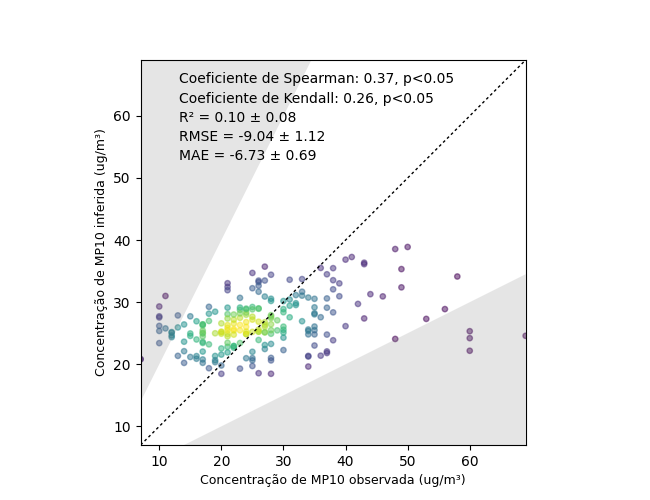
\includegraphics[width=\textwidth]{chapters/4-CALIBRAÇÃO MÚLTIPLOS SENSORES/Figuras/pm10-T-ML-Regression.png}
        \caption{Utilizando uma regressão linear multivariada considerando a temperatura obteve-se um R2 de 0.10 e $\rho$ de 0.37}
        \label{fig:data-pm10-T-reference-corr-MLR}
    \end{subfigure}
    \hfill
    \begin{subfigure}{0.49\textwidth}
        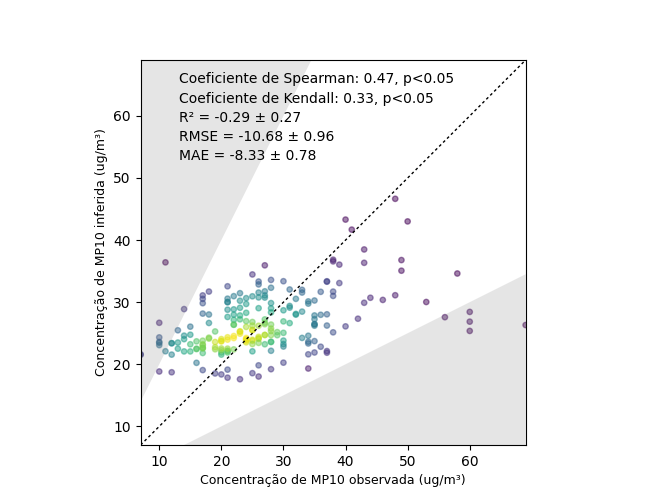
\includegraphics[width=\textwidth]{chapters/4-CALIBRAÇÃO MÚLTIPLOS SENSORES/Figuras/pm10-T-MLP-Regression.png}
        \caption{Utilizando uma rede neural Perceptron Multicamadas considerando a temperatura obtiveram-se valores de $\rho$ de 0.47 e 0.33}
        \label{fig:data-pm10-T-reference-corr-MLP}
    \end{subfigure}
\end{figure}

Como se observa, apenas o modelo de regressão linear com variáveis independentes temperatura e concentração medida pelo sensor OPC-N3 conseguiu explicar a variância na variável dependente, i.e. a concentração real. Os valores de R2 obtidos nas validações cruzadas realizadas para este modelo foram de 0.10 ± 0.08, e os coeficientes de correlação de Spearman e Kendall entre a concentração inferida na calibração e a concentração real foram de 0.37 e 0.26 respectivamente. Os erros RMSE e MAE estiveram próximos de 10 \(\mu g/m^3\), que é um valor relativamente baixo considerando a diferença elevada entre os valores de referência e as leituras do sensor (aproximadamente 10 vezes). De modo geral, os modelos não lineares que incluíram a temperatura como variável dependente, apresentaram melhorias na correlação entre a concentração real e a medida pelo sensor, com coeficientes de correlação de até 0.47. As Figuras \ref{fig:data-pm10-T-reference-corr-MLR} e \ref{fig:data-pm10-T-reference-corr-MLP} apresentam os resultados ao aplicar o modelo de regressão linear considerando leituras do sensor e temperatura e ao aplicar uma rede neural Perceptron Multicamadas considerando as mesmas variáveis de entrada.

\begin{figure}[h!]
    \centering
    \caption{Desempenho dos modelos de regressão aplicados para inferir as leituras de concentração de \acrshort{mp10} medidas pela estação de referência}
    \begin{subfigure}{0.9\textwidth}
        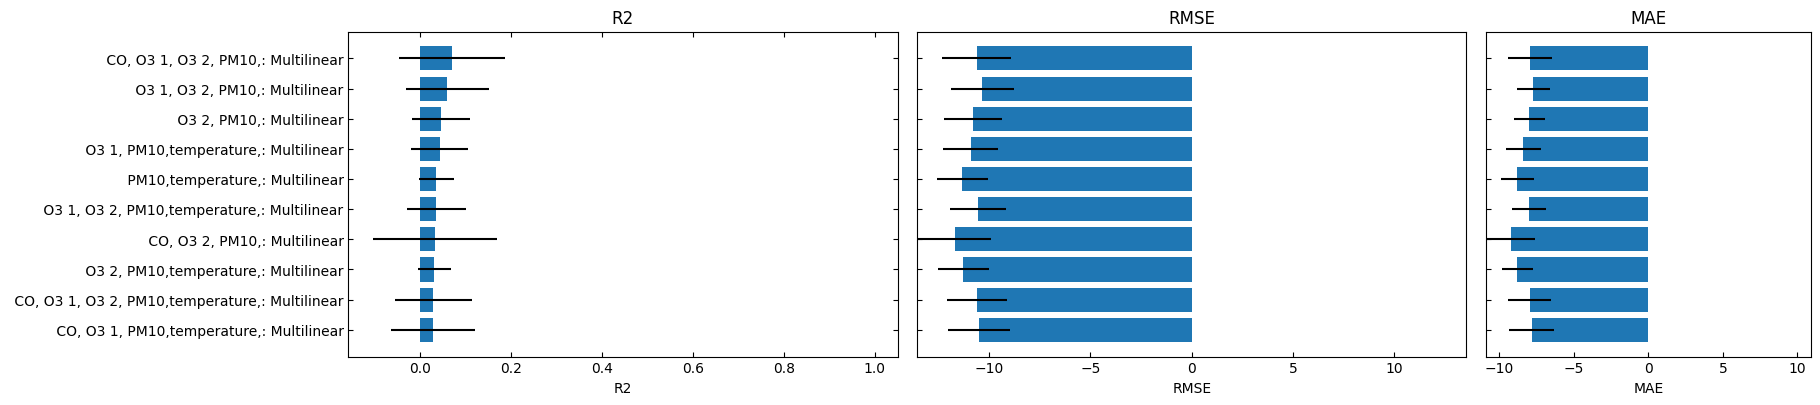
\includegraphics[width=\textwidth]{chapters/4-CALIBRAÇÃO MÚLTIPLOS SENSORES/Figuras/pm10-all-models-performance.png}
        \caption{Valores de R2, RMSE e MAE obtidos pelos 10 modelos com maiores valores de R2}
        \label{fig:data-pm10-all-models-performance}
    \end{subfigure}
    \begin{subfigure}{0.9\textwidth}
        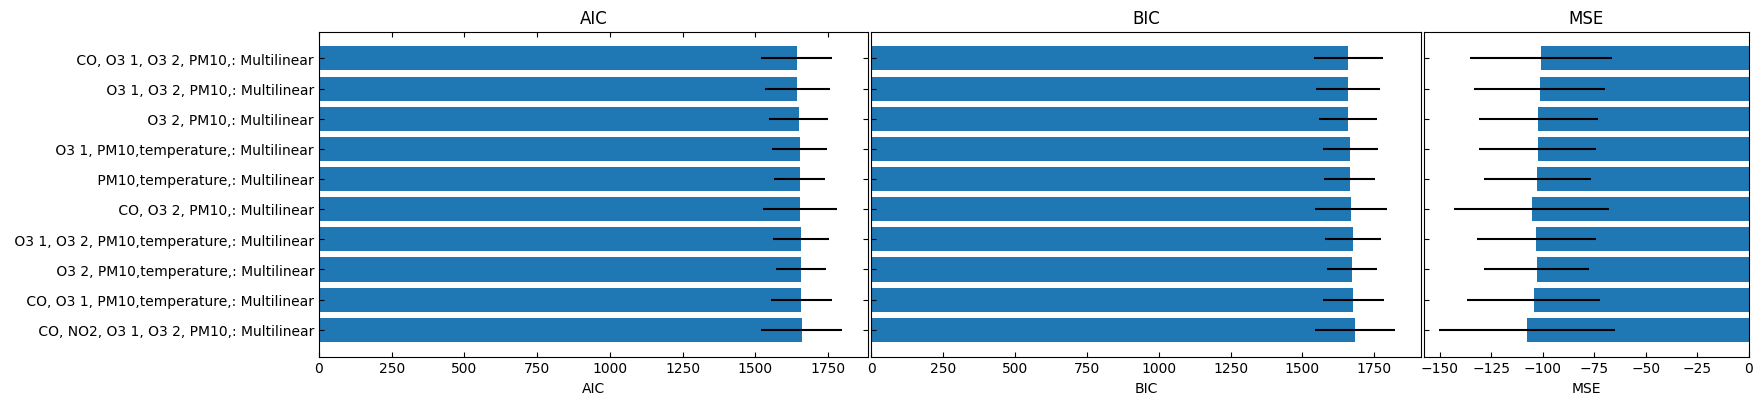
\includegraphics[width=\textwidth]{chapters/4-CALIBRAÇÃO MÚLTIPLOS SENSORES/Figuras/pm10-all-models-complexity.png}
        \caption{Modelos com menores valores de \acrshort{aic} e \acrshort{bic}}
        \label{fig:data-pm10-all-models-comlexity}
    \end{subfigure}
    \label{fig:data-pm10-all-models-performance-comlexity}
\end{figure}

% ----------------------------------------------------------
\section{Cálculo da concentração de MP10 a partir das leituras do arranjo de sensores de gases}
% ----------------------------------------------------------

A Figura \ref{fig:data-pm10-all-models-performance} apresenta os valores de R2 dos 10 melhores modelos de calibração calculados para as leituras de \acrshort{mp10}. Observa-se que os valores de R2 desses 10 modelos apresentaram valores de R2 em média positivos, com valores mínimos e máximos oscilando entre -0.1 e 0.2, todos obtidos a partir de regressões lineares. Com relação as variáveis de entrada observa-se maior variabilidade do que nos casos analisados anteriormente, mas em geral destaca-se a presença de sensores de \acrshort{o3} em 9 dos modelos e em segundo lugar da temperatura, presente em 6. Nenhum dos modelos incluiu leituras do sensor NO2-B43F. Com relação à complexidade dos modelos (Figura \ref{fig:data-pm10-all-models-performance-comlexity}) observa-se bastante coincidência com ranqueamento de R2. As Figuras \ref{fig:data-co-o31-o31-pm10-reference-PM10-corr-MLR} e \ref{fig:data-o31-o32-pm10-reference-PM10-corr-RF} mostram os resultados obtidos com os dois modelos com maior R2 médio, i.e.: regressões lineares com variáveis de entrada leituras de sensores CO-B4, OX-B431 (1 e 2) e sensor de \acrshort{mp10} OPC-N3, e leituras de sensores OX-B431 (1 e 2) e sensor de \acrshort{mp10} OPC-N3, respectivamente. As figuras mostram gráficos de dispersão entre os dados calibrados por esses modelos e as leituras de referência.

\begin{figure}[h]
    \centering
    \caption{Gráfico de dispersão das leituras do múltiplos sensores e a estação de referência para medição de \acrshort{mp10}}
    \begin{subfigure}{0.49\textwidth}
        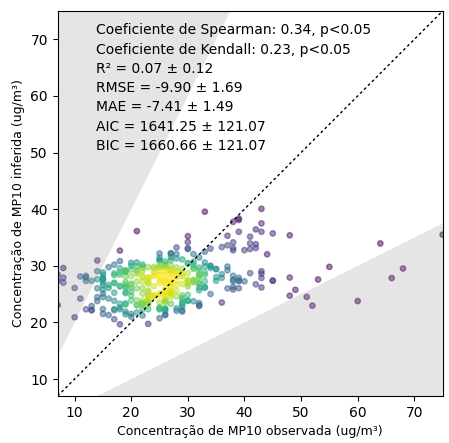
\includegraphics[width=\textwidth]{chapters/4-CALIBRAÇÃO MÚLTIPLOS SENSORES/Figuras/MP10-co-o31-o32-pm10-Multilinear-Regression.png}
        \caption{Utilizando modelo de regressão linear multivariado com variáveis independentes: leituras de sensores CO-B4, OX-B431 (1 e 2) e sensor de \acrshort{mp10} OPC-N3}
        \label{fig:data-co-o31-o31-pm10-reference-PM10-corr-MLR}
    \end{subfigure}
    \hfill
    \begin{subfigure}{0.49\textwidth}
        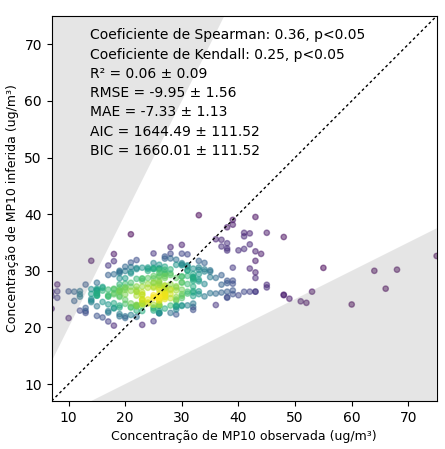
\includegraphics[width=\textwidth]{chapters/4-CALIBRAÇÃO MÚLTIPLOS SENSORES/Figuras/MP10-o31-o32-pm10-Multilinear-Regression.png}
        \caption{Utilizando modelo de regressão linear multivariado com variáveis independentes: leituras de sensores OX-B431 (1 e 2) e sensor de \acrshort{mp10} OPC-N3}
        \label{fig:data-o31-o32-pm10-reference-PM10-corr-RF}
    \end{subfigure}
\end{figure}


\section{Discussão}